\section{Context}

% Released on	10/10/2022, 4:46:17 PM	
% Last updated	
% 10/21/2022, 2:29:27 PM

The data was gathered from different sources including: my acquaintances, students of my faculty reached directly and through the Facebook (a popular social media platform) group consociating them, as well as my former employers who volunteered to help. Attempts at gathering data from Reddit (a popular internet forum) users failed.

I offered certain rewards to encourage participation in the research project, which included a chocolate treat (inspired by the article of Feitelson et. al. \cite{Fei22DeveloperNames}), small amount donated to a charity and obviously an unrestricted access to the tool with all of its features in the current version. Research suggests that such external incentives are not particularly effective \cite{Coh19AltruisticSurvey, Bru11DifferentMotivations}, nevertheless it is my way of showing appreciation to the contributors without generating potential conflicts with the law. Redistributing digital goods, for instance, may be seen as a compelling way of rewarding, but it goes against EULAs (end user agreements \cite{EULA}). The charity incentive, however, may prove quite effective especially in the current times \cite{Forbes22Philanthropy}.

The tool is build on the top of Visual Studio Code \ref{fig:embedded_extension} (a popular IDE-like code editing software) due to its prevalence within the programming realm \cite{StackOverflow22Survey}. Furthermore, VS Code is easily extensible with the common TypeScript/JavaScript (JavaScript is pervasive in web development and TypeScript is basically typed JavaScript) framework and I have professional experience in building web applications.

In the end the \texttt{MIMUW-MB-TT} plugin was released on 10th October 2022 and last updated on 21st October 2022. The participants were instructed not to uninstall the plugin for one week at bare minimum or better at least for two weeks. As of 20th November 2022 the plugin was downloaded 33 times and 13 packages of user data has been gathered. The tactic of directly speaking to the faculty students and driving them to download my plugin by rewarded them with a chocolate seem to result with the most prominent source of participants in the study.

\begin{figure}[htbp]
  \centering
  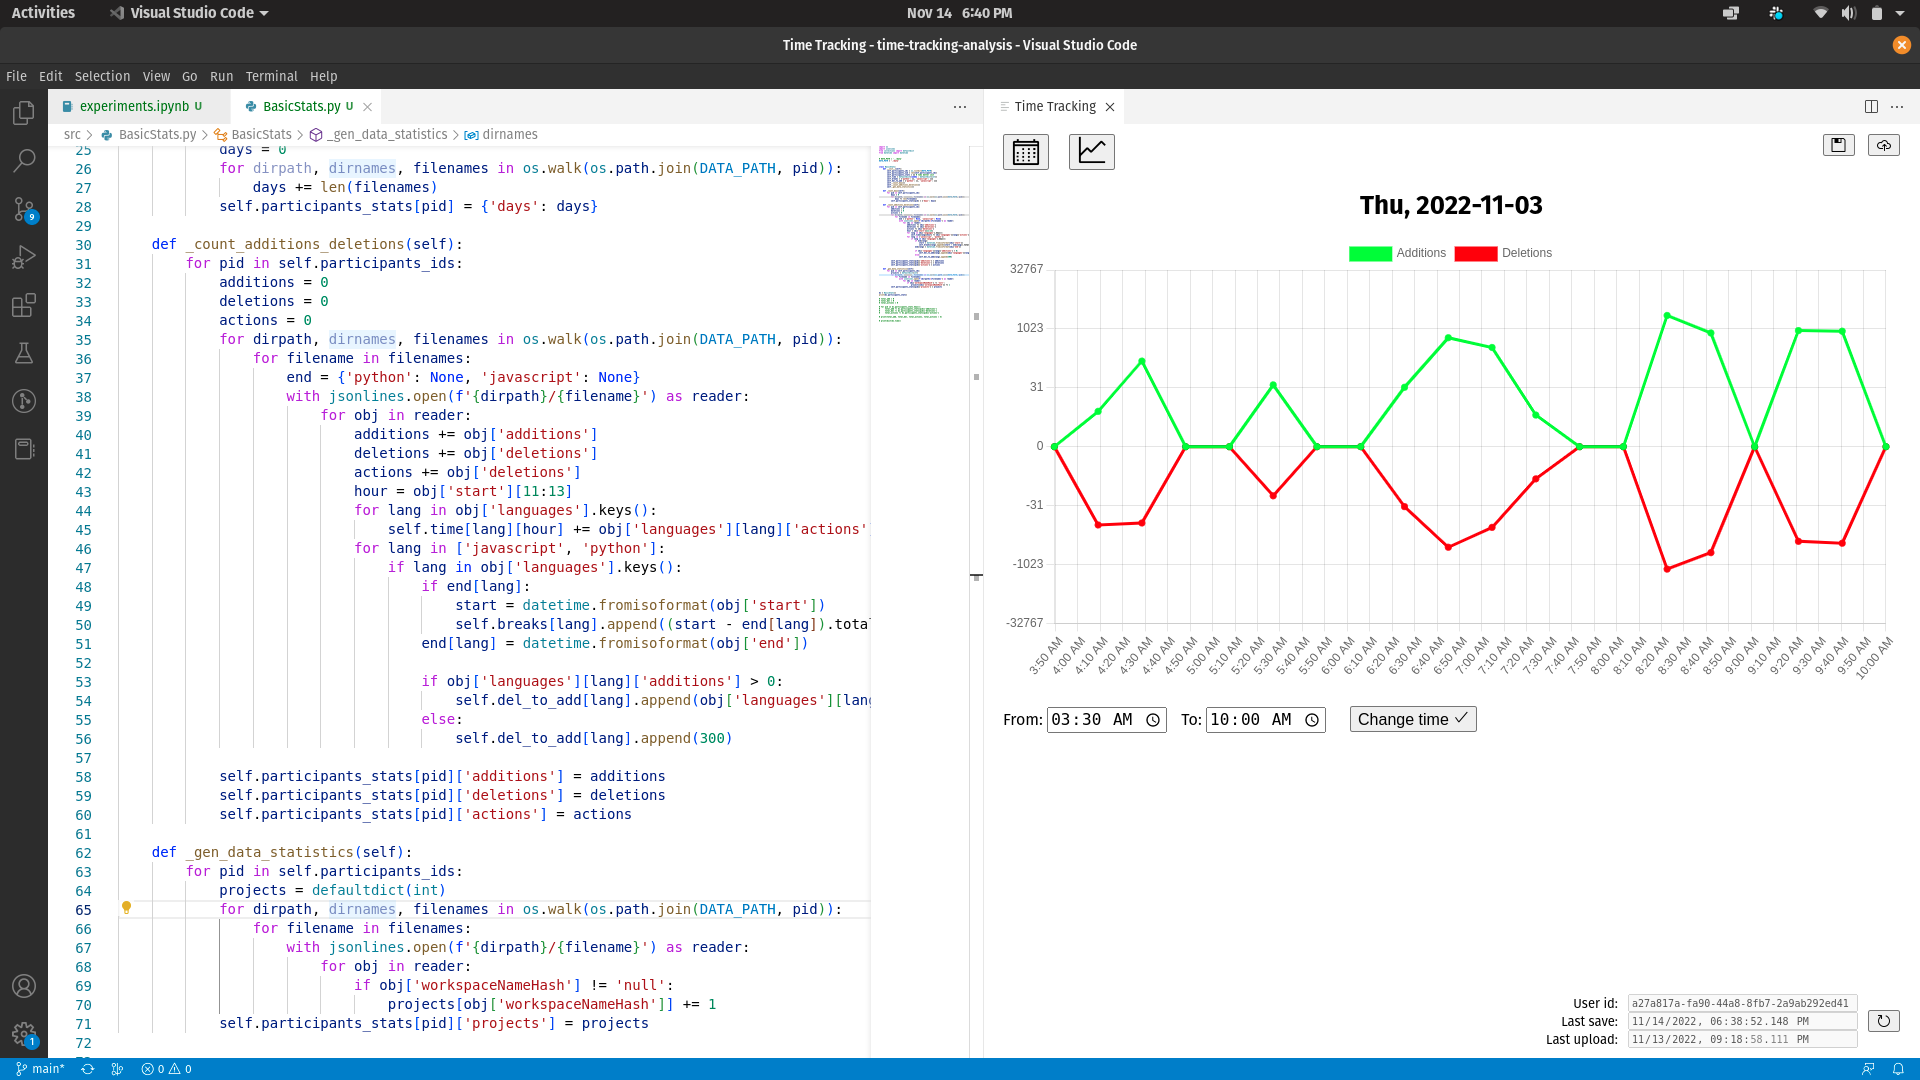
\includegraphics[scale=0.22]{chapters/methodology/graphics/extension-embedded.png}
  \caption{Extension embedded in Visual Studio Code}
  \label{fig:embedded_extension}
\end{figure}
